
% Copyright (c) 2015 - 2019 Mario Mlačak, mmlacak@gmail.com
% Licensed and published as Public Domain work.

% Tamoanchan Revisited chapter ========================================
\chapter*{Tamoanchan Revisited}
\addcontentsline{toc}{chapter}{Tamoanchan Revisited}

\begin{flushright}
\parbox{0.6\textwidth}{
\emph{I dream, therefore I exist. \\
\hspace*{\fill}{\textperiodcentered \textperiodcentered \textperiodcentered \hspace*{0.2em} August Strindberg} } }
\end{flushright}

\noindent
Tamoanchan Revisited is chess variant which is played on 22 x 22 board,
with white and bright cyan fields and light grey and grey pieces.
Star colors are yellow and bright red. In algebraic notation, columns
are enumerated from 'a' to 'v', and rows are enumerated from '1' to '22'.
A new piece is introduced, Serpent.

\clearpage % ..........................................................
% Serpent *************************************************************

\section*{Serpent}
\addcontentsline{toc}{section}{Serpent}

\noindent
\begin{wrapfigure}[11]{l}{0.4\textwidth}
\centering
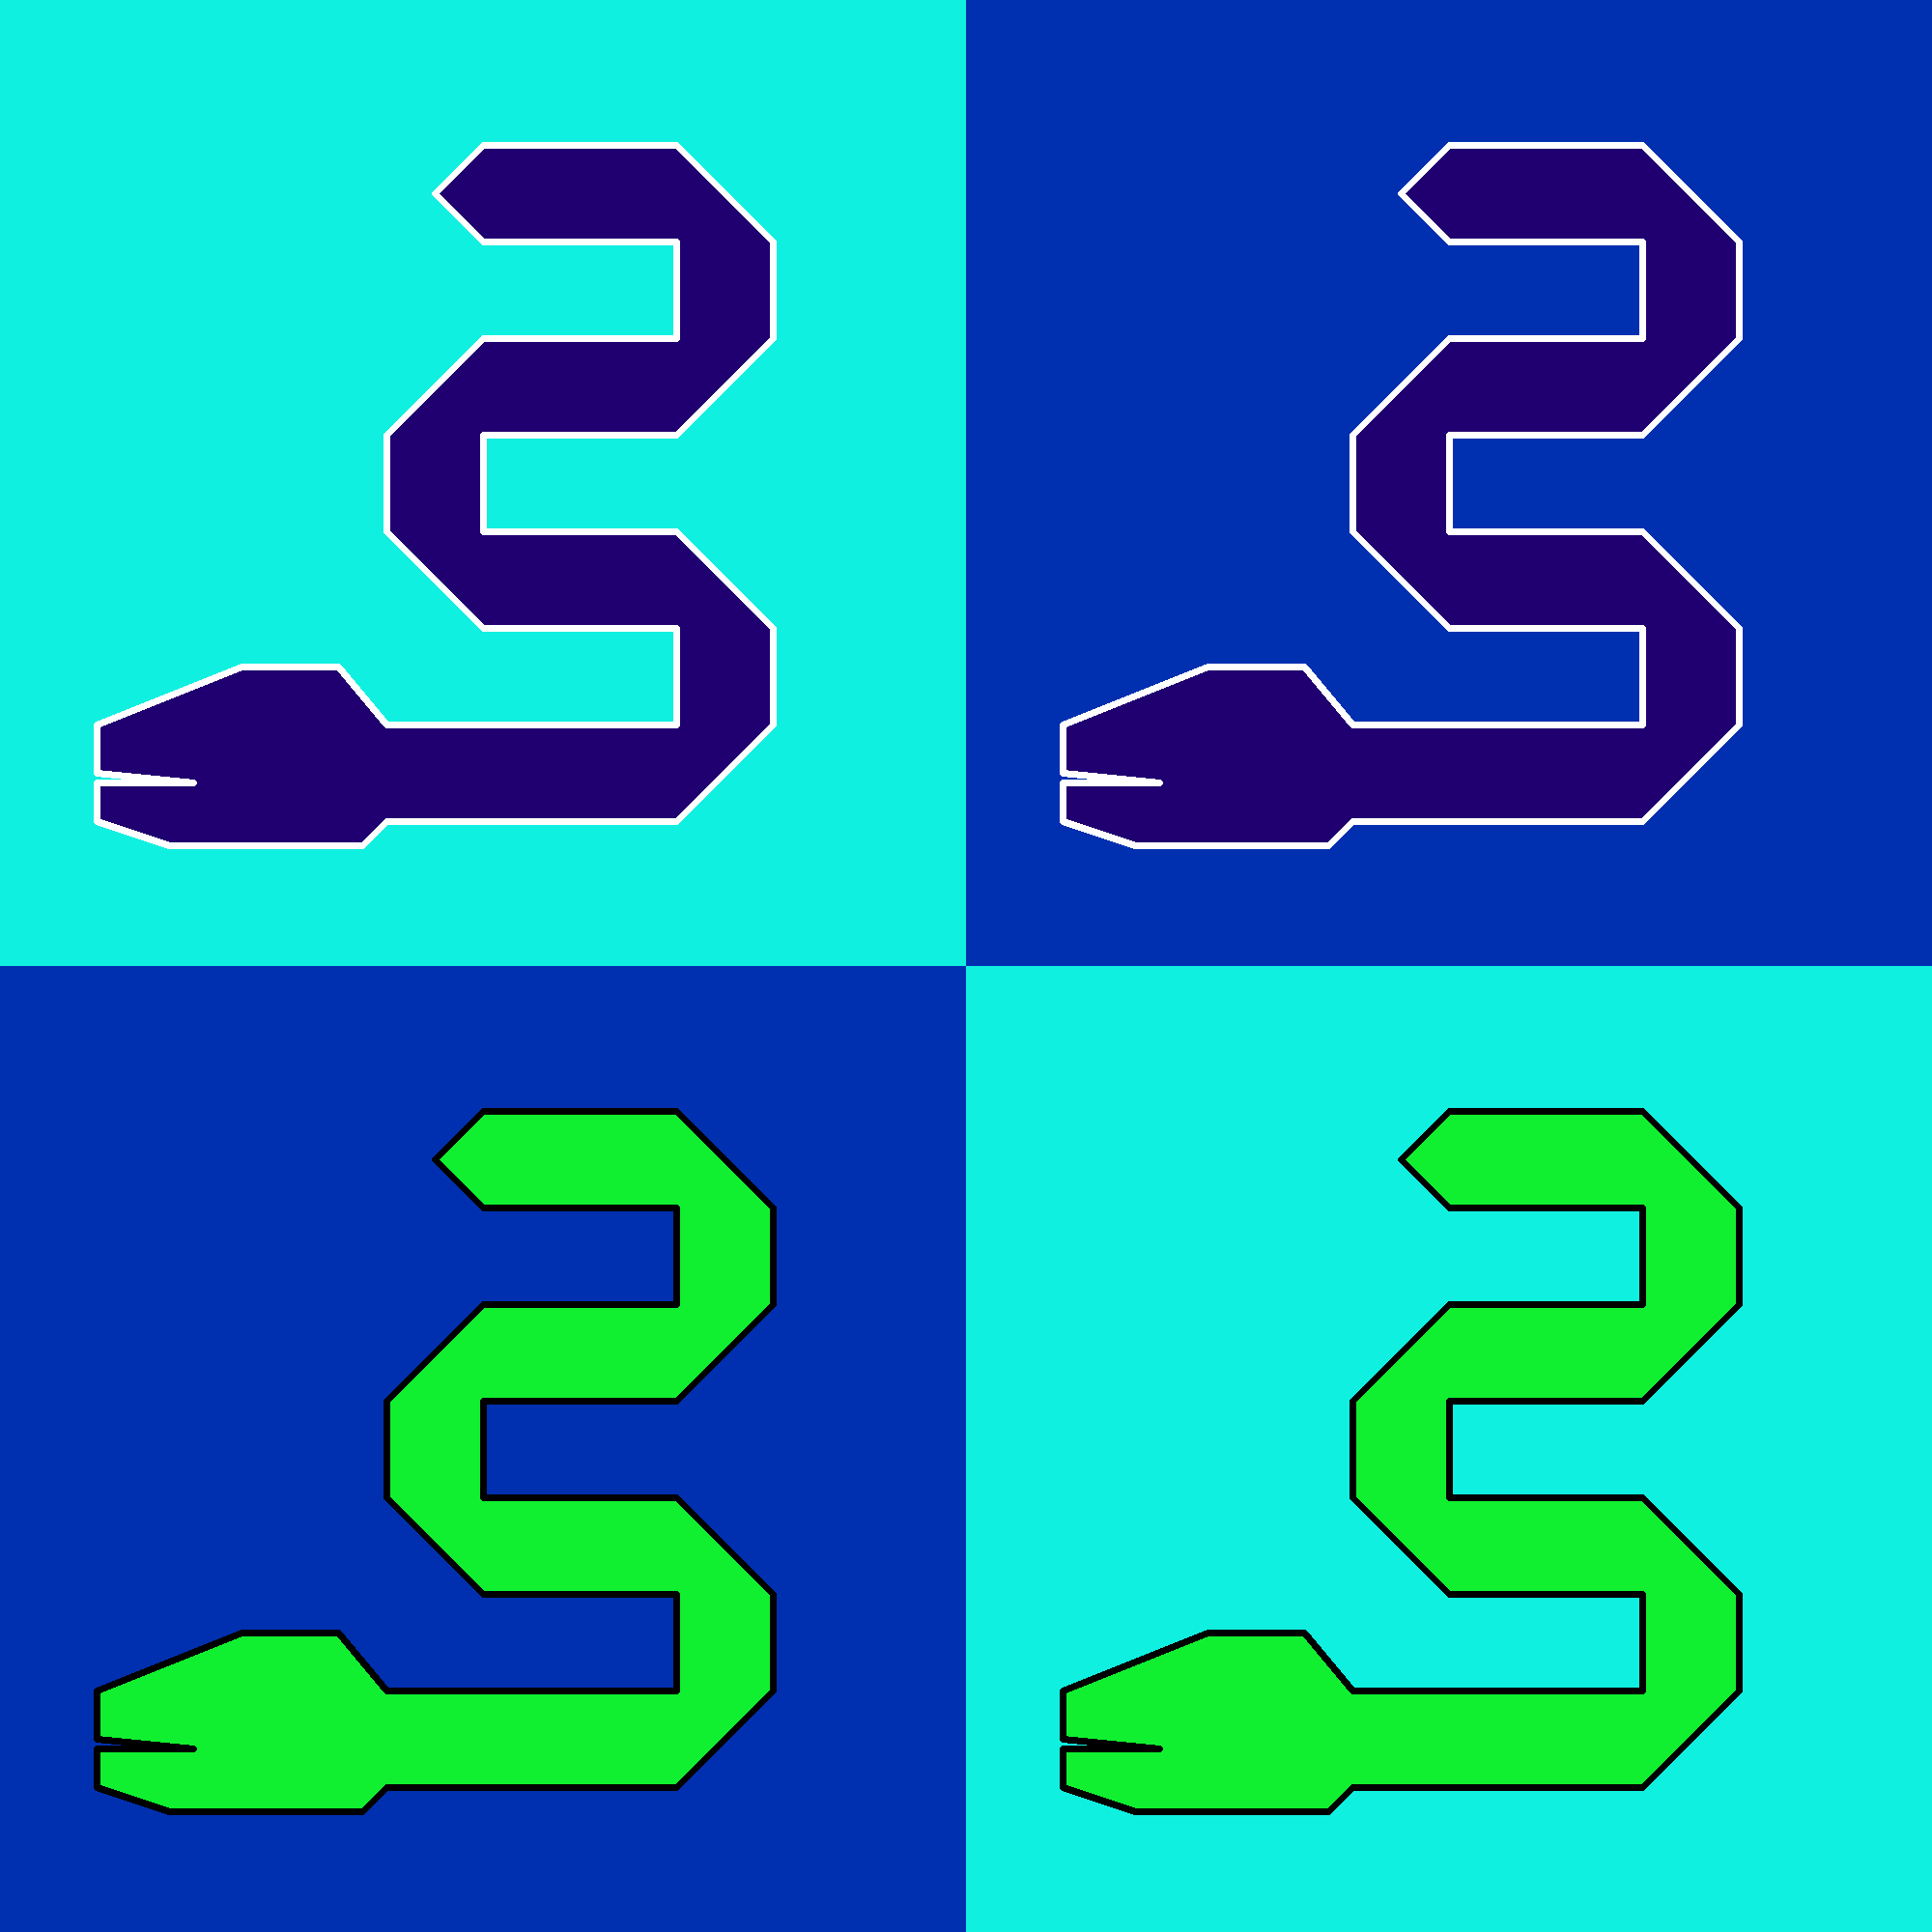
\includegraphics[width=0.4\textwidth, keepaspectratio=true]{pieces/13_serpent.png}
\caption{Serpent}
\label{fig:13_serpent}
\end{wrapfigure}
Serpent moves diagonaly one field at the time, after which it alternates
diagonal.

All step-fields are also capture-fields, Serpent would be able to activate
not just Wave, but also Pyramid on any of them.

Serpent can move no longer than for one third of board size, rounded up to
first whole number. In this variant that means Serpent can move for up to
8 fields, inclusively.

Alternatively, Serpent can also move one field vertically or horizontally
if it's unoccupied. This movement is a complete move of a player, and cannot
contain anything else.

In algebraic notation symbol for Serpent is ’S’.

% \vspace*{0.05\textheight}
\noindent
\begin{wrapfigure}{l}{0.4\textwidth}
\centering
\includegraphics[width=0.4\textwidth, keepaspectratio=true]{pieces/star/16_tamoanchan_revisited.png}
\caption{Star}
\label{fig:star/16_tamoanchan_revisited}
\end{wrapfigure}
Star colors in this variant are presented on the left.

\clearpage % ..........................................................
% Movement ------------------------------------------------------------

\subsection*{Movement}
\addcontentsline{toc}{subsection}{Movement}

\noindent
\begin{wrapfigure}[8]{l}{0.4\textwidth}
\centering
\includegraphics[width=0.363636363636\textwidth, keepaspectratio=true]{examples/16_tr/scn_tr_01_serpent_diagonals.png}
\caption{Diagonals}
\label{fig:scn_tr_01_serpent_diagonals}
\end{wrapfigure}
On its' first step Serpent can choose among any of the 4 diagonal fields,
i.e. either A or B diagonal.

On all subsequent steps Serpent has to alternate between diagonals.
Choice between 2 fields on a diagonal is independent of any previous choice.

\vspace*{0.04\textheight}
\noindent
\begin{wrapfigure}[5]{l}{0.4\textwidth}
\centering
\includegraphics[width=0.363636363636\textwidth, keepaspectratio=true]{examples/16_tr/scn_tr_02_serpent_1.png}
\caption{Step 1}
\label{fig:scn_tr_02_serpent_1}
\end{wrapfigure}
Starting position is marked S.

First step was taken onto upper-right field on diagonal B.
Next step has to be onto either field on diagonal A.

\vspace*{0.125\textheight}
\noindent
\begin{wrapfigure}[7]{l}{0.4\textwidth}
\centering
\includegraphics[width=0.363636363636\textwidth, keepaspectratio=true]{examples/16_tr/scn_tr_03_serpent_2.png}
\caption{Step 2}
\label{fig:scn_tr_03_serpent_2}
\end{wrapfigure}
Step taken by Serpent was onto upper-left field on A diagonal.

Next step has to be on diagonal B, chosen freely between the 2 fields,
regardless of choice made for the first step.

\clearpage % ..........................................................

\noindent
\begin{wrapfigure}[6]{l}{0.4\textwidth}
\centering
\includegraphics[width=0.363636363636\textwidth, keepaspectratio=true]{examples/16_tr/scn_tr_04_serpent_3.png}
\caption{Step 3}
\label{fig:scn_tr_04_serpent_3}
\end{wrapfigure}
Last step was on B diagonal, next step has to alternate again, onto A diagonal.

Field numbers counts steps to them, and also gathered momentum.

\vspace*{0.10\textheight}
\noindent
\begin{wrapfigure}[4]{l}{0.4\textwidth}
\centering
\includegraphics[width=0.363636363636\textwidth, keepaspectratio=true]{examples/16_tr/scn_tr_05_serpent_end.png}
\caption{End step}
\label{fig:scn_tr_05_serpent_end}
\end{wrapfigure}
Finished move with completely exhausted movement limit.

\clearpage % ..........................................................

\subsubsection*{Revisiting fields, loops}
\addcontentsline{toc}{subsubsection}{Revisiting fields, loops}

\noindent
\begin{wrapfigure}[8]{l}{0.4\textwidth}
\centering
\includegraphics[width=0.363636363636\textwidth, keepaspectratio=true]{examples/16_tr/scn_tr_07_serpent_loop_1.png}
\caption{Activating Pyramid}
\label{fig:scn_tr_07_serpent_loop_1}
\end{wrapfigure}
Starting with the same scene, only with added Pyramid, Serpent can
activate said Pyramid with momentum of 4.

There is nothing preventing Serpent to revisit already traversed fields,
and build up more momentum.

\vspace*{0.07\textheight}
\noindent
\begin{wrapfigure}[8]{l}{0.4\textwidth}
\centering
\includegraphics[width=0.363636363636\textwidth, keepaspectratio=true]{examples/16_tr/scn_tr_08_serpent_loop_end.png}
\caption{Building momentum}
\label{fig:scn_tr_08_serpent_loop_end}
\end{wrapfigure}
All revisited fields counts towards momentum each time they are traveled
over.

Here, fields are enumerated in visiting order, revisited fields are marked
blue. So, Serpent can now activate Pyramid with momentum of 8.

\clearpage % ..........................................................

\subsubsection*{Alternative movement}
\addcontentsline{toc}{subsubsection}{Alternative movement}

\noindent
\begin{wrapfigure}[9]{l}{0.4\textwidth}
\centering
\includegraphics[width=0.363636363636\textwidth, keepaspectratio=true]{examples/16_tr/scn_tr_06_serpent_neighbors.png}
\caption{Alternative movement}
\label{fig:scn_tr_06_serpent_neighbors}
\end{wrapfigure}
Serpent's alternative move is a way to change color of accessible fields,
provided that destination field is empty, or occupied by a Star.

Color-changing fields are all fields immediately neighboring starting
location, either horizontally or vertically, but not diagonaly.

\clearpage % ..........................................................

\subsubsection*{Out-of-board steps}
\addcontentsline{toc}{subsubsection}{Out-of-board steps}

\vspace*{-1.0\baselineskip}
\noindent
\begin{figure}[!h]
% \begin{figure}[!t]
\includegraphics[width=1.0\textwidth, keepaspectratio=true]{examples/16_tr/scn_tr_09_serpent_out_of_board.png}
\caption{Serpent out-of-board steps}
\label{fig:scn_tr_09_serpent_out_of_board}
% \centering
\end{figure}

Here, light grey fields are virtual fields extending existing chessboard.
For Serpent, it's illegal to step outside chessboard, and all subsequent
steps are also illegal. That means, Serpent cannot reach fields 1 through
4 with selected path, even though it would end movement on the chessboard.

\clearpage % ..........................................................

\subsubsection*{Teleporting Serpent}
\addcontentsline{toc}{subsubsection}{Teleporting Serpent}

\vspace*{-1.0\baselineskip}
\noindent
\begin{figure}[!h]
% \begin{figure}[!t]
\includegraphics[width=1.0\textwidth, keepaspectratio=true]{examples/16_tr/scn_tr_10_teleport_serpent_1.png}
\caption{Teleporting Serpent}
\label{fig:scn_tr_10_teleport_serpent_1}
% \centering
\end{figure}

Serpent teleports to any empty portal-field near Star in opposite color
(here, fields 1 -- 6), just like
\hyperref[fig:scn_n_02_teleport_init]{any other piece, except Wave}.
Serpent is bound to fields in one color, similar to Bishop. Teleporting
Serpent presents opportunity to change color of available fields (here,
portal-fields 2, 5), also
\hyperref[fig:scn_n_14_teleport_bishop]{similar to Bishop}.

\clearpage % ..........................................................

\vspace*{-1.0\baselineskip}
\noindent
\begin{figure}[!h]
% \begin{figure}[!t]
\includegraphics[width=1.0\textwidth, keepaspectratio=true]{examples/16_tr/scn_tr_11_teleport_serpent_2.png}
\caption{Color-changing step}
\label{fig:scn_tr_11_teleport_serpent_2}
% \centering
\end{figure}

Serpent can also teleport by performing color-changing step. This also
gives opportunity for Serpent to change color of accessible fields. Note,
color changing portal-fields (here, fields 1, 3, 4, 6) are switched
compared to previous example.

% ------------------------------------------------------------ Movement
\clearpage % ..........................................................
% Activating Wave -----------------------------------------------------

\subsection*{Activating Wave}
\addcontentsline{toc}{subsection}{Activating Wave}

% \vspace*{-1.0\baselineskip}
\noindent
\begin{wrapfigure}[3]{l}{0.4\textwidth}
\centering
\includegraphics[width=0.363636363636\textwidth, keepaspectratio=true]{examples/16_tr/scn_tr_12_serpent_activating_wave.png}
\caption{Activating}
\label{fig:scn_tr_12_serpent_activating_wave}
\end{wrapfigure}
Serpent can activate Wave on its' step-fields only, it cannot activate Wave
on \hyperref[fig:scn_tr_06_serpent_neighbors]{color-changing fields}.

\vspace*{7.0\baselineskip}
\noindent
\begin{wrapfigure}[2]{l}{0.4\textwidth}
\centering
\includegraphics[width=0.363636363636\textwidth, keepaspectratio=true]{examples/16_tr/scn_tr_13_serpent_activated_wave.png}
\caption{Activated}
\label{fig:scn_tr_13_serpent_activated_wave}
\end{wrapfigure}
Activated Wave can freely choose any diagonal field for its' first step.

\vspace*{8.0\baselineskip}
\noindent
\begin{wrapfigure}[2]{l}{0.4\textwidth}
\centering
\includegraphics[width=0.363636363636\textwidth, keepaspectratio=true]{examples/16_tr/scn_tr_14_serpent_activated_wave_step_1.png}
\caption{First step}
\label{fig:scn_tr_14_serpent_activated_wave_step_1}
\end{wrapfigure}
After first step, Wave must choose next step from the other diagonal.

\clearpage % ..........................................................

\noindent
\begin{figure}[!h]
% \begin{figure}[!t]
\includegraphics[width=1.0\textwidth, keepaspectratio=true]{examples/16_tr/scn_tr_15_serpent_activated_wave_ply.png}
\caption{Activated Wave ply}
\label{fig:scn_tr_15_serpent_activated_wave_ply}
% \centering
\end{figure}

Once the two directions are chosen, Wave has to alternate between them.
So, Wave cannot change given directions, even if it's on a proper diagonal.
E.g. upon reaching field 6, it's illegal for Wave to choose different
direction on B diagonal.

Unlike Serpent, Wave is not limited by number of steps. So, Wave can repeat
alternating between 2 chosen directions to the end of the chessboard.

\clearpage % ..........................................................

\subsubsection*{Out-of-board steps}
\addcontentsline{toc}{subsubsection}{Out-of-board steps}

\vspace*{-1.0\baselineskip}
\noindent
\begin{figure}[!h]
% \begin{figure}[!t]
\includegraphics[width=1.0\textwidth, keepaspectratio=true]{examples/16_tr/scn_tr_16_wave_out_of_board.png}
\caption{Wave out-of-board steps}
\label{fig:scn_tr_16_wave_out_of_board}
% \centering
\end{figure}

Again, light grey fields are virtual fields extending existing chessboard.
Wave activated by Serpent can step outside of a board, as long as its' ply
ends on a board. Here, all enumerated step-fields 1 through 8 are reachable
by Wave, even though it stepped outside of the board. It is illegal for any
piece, including Wave, to end its' ply outside of a board.

\clearpage % ..........................................................

\subsection*{Teleporting Wave}
\addcontentsline{toc}{subsection}{Teleporting Wave}

\vspace*{-1.0\baselineskip}
\noindent
\begin{figure}[!h]
% \begin{figure}[!t]
\includegraphics[width=1.0\textwidth, keepaspectratio=true]{examples/16_tr/scn_tr_17_off_board_teleport_wave.png}
\caption{Teleporting off-board Wave}
\label{fig:scn_tr_17_off_board_teleport_wave}
% \centering
\end{figure}

\huge{TODO}
\normalsize{}

Activated \& teleported Wave ... by Serpent on board edge ... continuity of alterations between step directions

\clearpage % ..........................................................

\vspace*{-1.0\baselineskip}
\noindent
\begin{figure}[!h]
% \begin{figure}[!t]
\includegraphics[width=1.0\textwidth, keepaspectratio=true]{examples/16_tr/scn_tr_18_teleported_wave_on_board.png}
\caption{Teleported Wave}
\label{fig:scn_tr_18_teleported_wave_on_board}
% \centering
\end{figure}

...

\clearpage % ..........................................................

\vspace*{-1.0\baselineskip}
\noindent
\begin{figure}[!h]
% \begin{figure}[!t]
\includegraphics[width=1.0\textwidth, keepaspectratio=true]{examples/16_tr/scn_tr_19_on_board_teleport_wave.png}
\caption{Teleporting Wave}
\label{fig:scn_tr_19_on_board_teleport_wave}
% \centering
\end{figure}

\huge{BUG}
\normalsize{}

TODO :: BUG :: generator overflows by 1, count is half it should be (actually, 15)

\clearpage % ..........................................................

\vspace*{-1.0\baselineskip}
\noindent
\begin{figure}[!h]
% \begin{figure}[!t]
\includegraphics[width=1.0\textwidth, keepaspectratio=true]{examples/16_tr/scn_tr_20_teleported_wave_off_board.png}
\caption{Teleporting Wave}
\label{fig:scn_tr_20_teleported_wave_off_board}
% \centering
\end{figure}

...

% ----------------------------------------------------- Activating Wave
% ************************************************************* Serpent
\clearpage % ..........................................................

\section*{Promotion}
\addcontentsline{toc}{section}{Promotion}

Promotion is non enforced, delayed variety, i.e. it's the same as in
\hyperref[sec:Age of Aquarius/Promotion]{previous chess variant}, Age of Aquarius.

Promotion in this variant is polygamous, more than one Queen in the same color
can be present on chessboard at any given time.

\clearpage % ..........................................................

\section*{En passant}
\addcontentsline{toc}{section}{En passant}

\noindent
\begin{wrapfigure}{l}{0.4\textwidth}
\centering
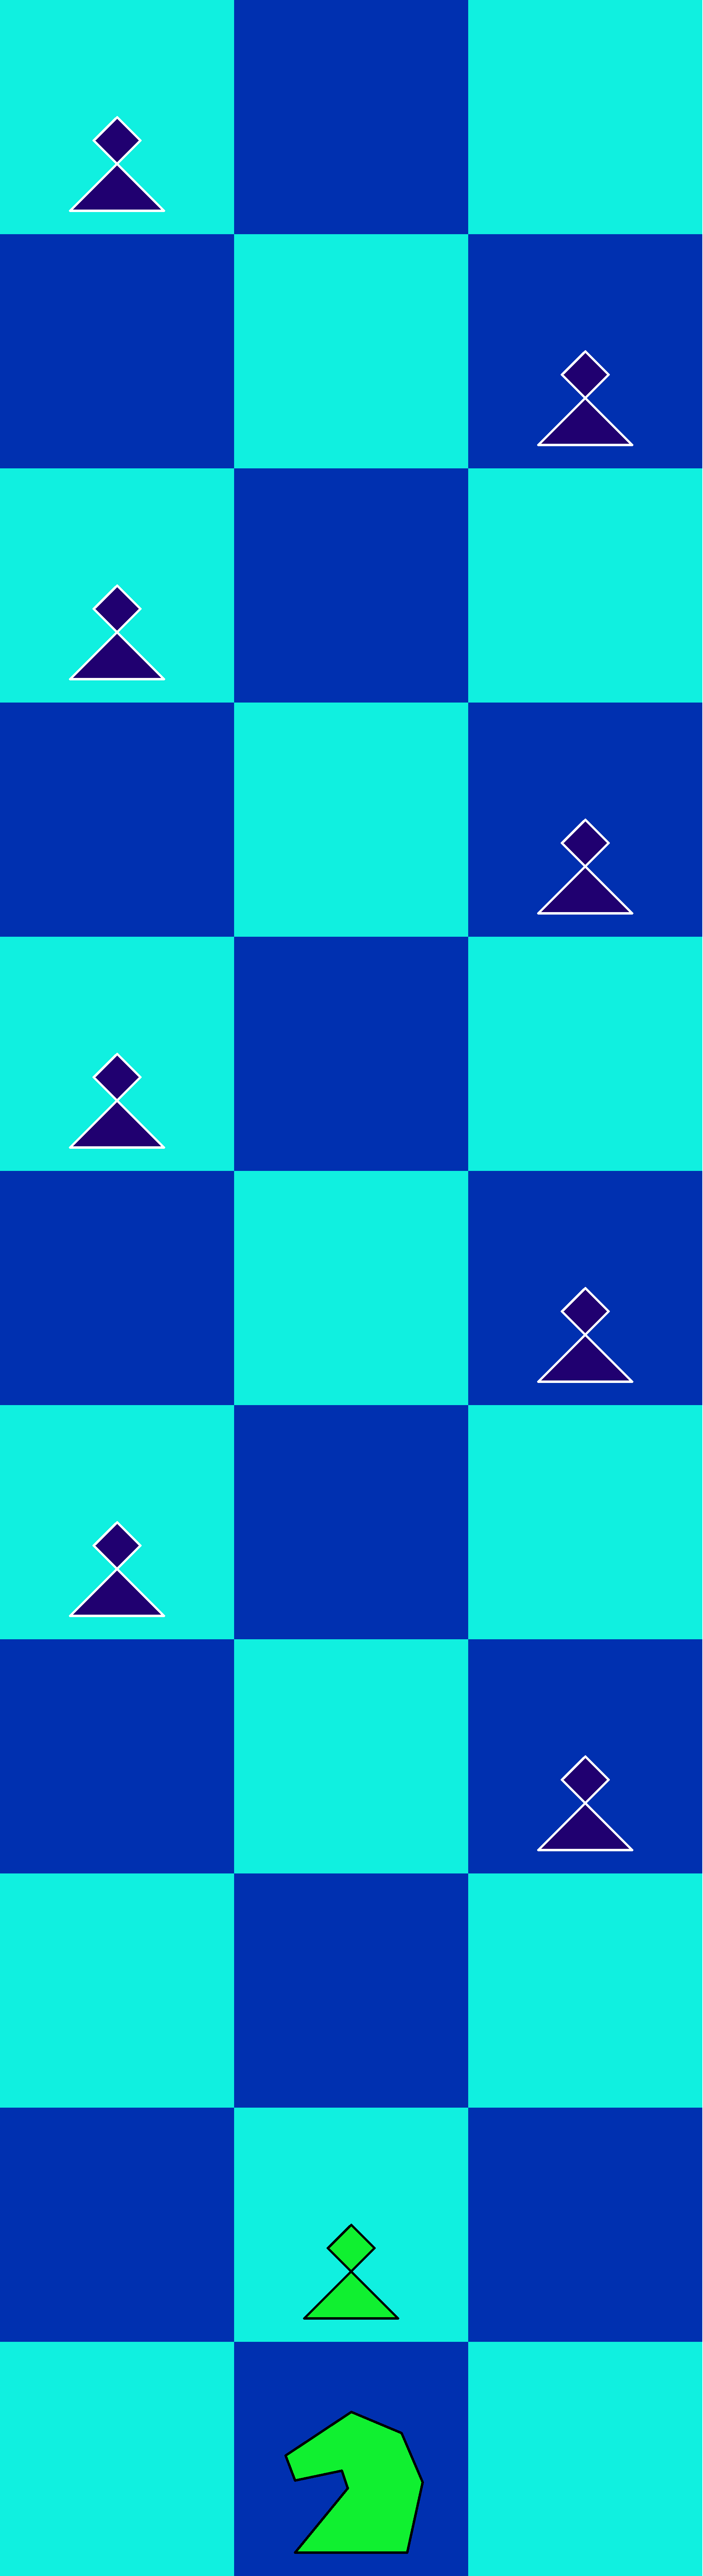
\includegraphics[width=0.136363636364\textwidth, keepaspectratio=true]{en_passants/16_tamoanchan_revisited_en_passant.png}
\caption{En passant}
\label{fig:16_tamoanchan_revisited_en_passant}
\end{wrapfigure}
Rush and en passant are identical to those in Classic Chess, only difference
is that Pawn can now move longer on initial turn, up to 9 fields in this
variant.

\clearpage % ..........................................................

\section*{Castling}
\addcontentsline{toc}{section}{Castling}

Castling is the same as in Classical Chess, only difference is that King can move between 2 and 8 fields across.
All other constraints from Classical Chess still applies.

\noindent
\begin{figure}[!h]
% \begin{figure}[!t]
\includegraphics[width=1.0\textwidth, keepaspectratio=true]{castlings/16_tr/tamoanchan_revisited_castling.png}
\caption{Castling}
\label{fig:tamoanchan_revisited_castling}
% \centering
\end{figure}

In example above, all valid King's castling moves are numbered.

\noindent
\begin{figure}[!h]
% \begin{figure}[!t]
\includegraphics[width=1.0\textwidth, keepaspectratio=true]{castlings/16_tr/tamoanchan_revisited_castling_left_03.png}
\caption{Castling short left}
\label{fig:tamoanchan_revisited_castling_left_03}
% \centering
\end{figure}

In this example King was castling short to the left. Initial King's position is marked with "K".
After castling is finished, left Rook ends up at field immediately right to the King.

\clearpage % ..........................................................

\section*{Initial setup}
\addcontentsline{toc}{section}{Initial setup}

Compared to initial setup of Hemera's Dawn, Serpent is inserted between Knight and Centaur
symmetrically, on both sides of chessboard. This can be seen in the image below:

\noindent
% \begin{figure}[t]
\begin{figure}[h]
\includegraphics[width=1.0\textwidth, keepaspectratio=true]{boards/16_tamoanchan_revisited.png}
\caption{Tamoanchan Revisited board}
\label{fig:16_tamoanchan_revisited}
% \centering
\end{figure}

\clearpage % ..........................................................
% ======================================== Tamoanchan Revisited chapter
